\documentclass[11pt, openany]{article}

\usepackage[T1]{fontenc}
\usepackage[utf8]{inputenc}
\usepackage[english, italian]{babel}
\usepackage{cancel}

\usepackage{hyperref}
\hypersetup{colorlinks=true,
	linkcolor=black,
	citecolor= black,
	filecolor=magenta,
	urlcolor=cyan,
}

\usepackage{geometry}
\geometry{
	a4paper,
	top=2.5cm,
	bottom=2cm,
	left=1.5cm,
	right=1.5cm,
	heightrounded,
	bindingoffset=5mm
}

\usepackage{amsmath}
\usepackage{amssymb}
\usepackage{amsthm}
\usepackage{tabularx}
\usepackage{booktabs}
\usepackage{caption}
\captionsetup{font = smaller}
\usepackage{enumitem}
\usepackage{blindtext}
\usepackage[x11names]{xcolor}
\usepackage{tcolorbox}
\usepackage{graphicx}
\usepackage{pdfpages}
\usepackage[export]{adjustbox}
\usepackage{cleveref}
\usepackage{multirow}
\usepackage{lipsum}



\theoremstyle{definition}
\newtheorem*{defn}{Definizione}
\newtheorem{exe}{Esercizio}[section]
\newtheorem{esem}{Esempio}[section]
\theoremstyle{plain}
\theoremstyle{remark}
\newtheorem*{warn}{ATTENZIONE}
\newtheorem*{svol}{Svolgimento}

\setcounter{secnumdepth}{-1}
\setcounter{tocdepth}{4}


\setlist[itemize]{nosep}
\usepackage{helvet}
\renewcommand{\familydefault}{\sfdefault}


 
\title{Relazione progetto di\\\textbf{Basi di Dati e \\Sistemi Informativi}\\A.A. 2022/2023}
\author{Diciotti \hfill Matteo \\ 7072181 \and Manucci \hfill Agostino \\ 7084379}
\date{\today}

\begin{document}
	\maketitle
	\hrule
	
	\part{}
		\paragraph{Titolo}
			Relazione progetto A.A. 2022/2023 di Basi di Dati e Sistemi Informativi
		\paragraph{Autori}
			\footnotesize Lista degli autori ordinata per numero di matricola\\
			\normalsize
			\begin{tabularx}{\textwidth}[t]{p{4.5cm} p{3.5cm} p{2.5cm} r}
				\textbf{Matricola} 	& 	\textbf{Cognome} 	& 	\textbf{Nome} 	& \textbf{e-mail} 					\\\toprule
				7072181				&	Diciotti			&	Matteo			&	matteo.diciotti@stud.unifi.it	\\
				7084379				&	Mannucci			&	Agostino		&	agostino.mannucci@stud.unifi.it
			\end{tabularx}

		\paragraph{Obiettivo}
			Obiettivo del progetto è la realizzazione, per fini accademici, di una base di dati a partire dall'identificazione di una richiesta realmente proponibile, seguita dalla fase di progettazione concettuale cui dovrà succedere la fase di progettazione logica e quindi la realizzazione in MySQL.

		\paragraph{Introduzione al progetto}
			La realizzazione di una base di dati prevede che sia definita rigorosamente una \underline{richiesta}, pilastro attorno cui si sviluppa il database passando da alcune importanti fasi: una fase di studio, concentrata principalmente nella fase di \textit{progettazione concettuale}, una fase di analisi, suddivisa tra la fase di \textit{progettazione concettuale} e la fase di \textit{progettazione logica}, ed infine una fase di sviluppo, concentrata nella fase di \textit{progettazione logica} e nella realizzazione in linguaggio \textit{MySQL}.\\
			La creazione della base proposta parte dalla scrittura di una richiesta completa e precisa, affinché fosse plausibile che la fase preliminare, comprendente il confronto col richiedente, fosse già avvenuta proficuamente avendo quindi predefinito le specifiche necessarie ed i dettagli importanti per il cliente. Nella progettazione siamo quindi partiti da una richiesta che non dovesse essere modificata ulteriormente ma che potesse considerarsi definitiva e quindi immediatamente appetibile per le fasi di progettazione suddette, bacino nozionistico del corso.\\
			La stesura della relazione segue a grandi linee l'ordine con cui sono state affrontate le varie fasi di progettazione e realizzazione: \textit{analisi della richiesta}, \textit{analisi dei termini}, \textit{traduzione del testo} e \textit{creazione del glossario dei termini}, dopodiché è stato \textit{creato il modello ER} (questa prima parte rappresenta la \underline{progettazione concettuale}). Per quanto concerne la fase di \underline{progettazione logica} sono state eseguite le scelte implementative durante le procedure di \textit{eliminazione delle gerarchie}, \textit{eliminazione degli attributi multi-valore} e nella \textit{scelta degli identificatori principali}, giungendo infine al \textit{modello ER ristrutturato}. Da questo è stato quindi definito passo-passo lo schema logico, fino a giungere allo \underline{schema logico completo} a pagina \pageref{tab:schema logico}.\\
			La fase di realizzazione in MySQL viene affrontata nella presente relazione suddividendo lo script in sezioni tematiche, ovvero in cinque parti che rappresentano i meccanismi focali dell'implementazione:
			\begin{itemize}
				\item Creazione e popolamento delle tabelle
				\item Interrogazioni
				\item Procedure e funzioni
				\item Viste
				\item Trigger
			\end{itemize}
			
	\part{Richiesta}
		Una società che organizza tornei di calcio a 5 e a 7 è presente nel territorio toscano con tornei attivi nella città di Firenze e nelle zone limitrofe.\\\\
		Di questi tornei la società desidera mantenere informazioni relative alle fasi di gioco, alle squadre partecipanti, ai giocatori che compongono le formazioni e alle partite.\\
		I tornei sono identificati tramite un codice e sono caratterizzati da un nome, da un’edizione, dalla tipologia di gioco (calcio a 5 o a 7) e dalla categoria di genere (maschile, femminile o mista).\\
		Ogni torneo può essere suddiviso in più fasi di gioco (tipicamente da 1 a 3), le quali si distinguono per la modalità di organizzazione degli scontri tra le squadre (a gironi o ad eliminazione diretta) e che sono caratterizzate dal nome della fase e da un numero rappresentante la quantità di scontri tra due squadre	nella fase. Alle fasi possono corrispondere uno o più insiemi di squadre partecipanti e un gruppo di
		giornate di gioco, che rappresentano i turni della fase.\\
		Gli insiemi di squadre, identificati dalla fase a cui appartengono e dal nome dell'insieme, raggruppano	le formazioni partecipanti a quella fase.\\
		Le giornate di gioco calendarizzano le partite di una fase e possiedono su queste i vincoli imposti alla modalità di organizzazione degli scontri (a gironi o ad eliminazione diretta). Le giornate sono identificate dalla fase a cui appartengono e dal numero della giornata.\\
		In particolare è rilevante per ogni partita conoscere la squadra di casa e la squadra ospite, la data di gioco, il campo, l’arbitro che dirige la gara e al punteggio finale.\\
		Per ogni partita la società ha interesse a mantenere le statistiche sui giocatori che hanno effettuato azioni rilevanti in quella partita (gol fatti, assist effettuati, espulsioni, ammonizioni), mentre le squadre si distinguono per il nome, la tipologia di calcio a cui giocano e il genere dei giocatori che la compongono.
		La società richiede inoltre che sia mantenuta l’informazione sul campo di casa il quale è contraddistinto dagli altri campi attraverso l’indirizzo. I campi possiedono comunque un nome proprio e un recapito.
		Le persone tesserate alla società si suddividono in due tipologie: i giocatori e gli arbitri i quali condividono un numero di tessera univoco per ogni tesserato.\\
		Di tutti gli iscritti si conoscono nome e cognome, data di nascita e genere, mentre per i giocatori si conosce, qualora partecipino a qualche torneo, anche la squadra a con la quale gareggiano ed il relativo numero di maglia.
	
	\part{Progettazione Concettuale}
		\section{Analisi della richiesta}
			Si procede all’analisi della richiesta evidenziando:
			\begin{itemize}
				\item in \textit{corsivo} i termini ambigui o imprecisi;
				\item \underline{sottolineati} i termini con i quali si esprimono concetti diversi;
				\item in \textbf{grassetto} i termini concettualmente equivalenti, distinguendo successivamente le equivalenze.
			\end{itemize}
			
			\begin{tcolorbox}[width=\textwidth,colback={Cornsilk2}]\label{text:analisi richiesta}
				Una società che organizza tornei di calcio a 5 e a 7 è presente nel territorio toscano con tornei attivi nella città di Firenze e nelle zone limitrofe.\\\\
				Di questi tornei la società desidera mantenere informazioni relative alle fasi di gioco, alle \textbf{squadre} \underline{partecipanti}, ai giocatori che compongono le \textbf{formazioni} e alle \textbf{partite}.\\
				I tornei sono identificati tramite un codice e sono caratterizzati da un \underline{nome}, da un’\textit{edizione}, dalla \underline{tipologia} di gioco (calcio a 5 o a 7) e dalla categoria di \underline{genere} (maschile, femminile o mista).\\
				Ogni torneo può essere suddiviso in più fasi di gioco (tipicamente da 1 a 3), le quali si distinguono per la modalità di organizzazione degli \textbf{scontri} tra le squadre (a gironi o ad eliminazione diretta) e che sono caratterizzate dal \underline{nome} della fase e da un \underline{numero} rappresentante la quantità di scontri tra due squadre	nella fase. Alle fasi possono corrispondere uno o più insiemi di squadre partecipanti e un gruppo di
				giornate di gioco, che rappresentano i turni della fase.\\
				Gli insiemi di squadre, identificati dalla fase a cui appartengono e dal \underline{nome} dell'insieme, raggruppano	le formazioni partecipanti a quella fase.\\
				Le giornate di gioco calendarizzano le partite di una fase e possiedono su queste i vincoli imposti alla modalità di organizzazione degli scontri (a gironi o ad eliminazione diretta). Le giornate sono identificate dalla fase a cui appartengono e dal \underline{numero} della giornata.\\
				In particolare è rilevante per ogni partita conoscere la squadra di casa e la squadra ospite, la \underline{data} di gioco, il \underline{campo}, l’arbitro che dirige la \textbf{gara} e al \textit{punteggio} finale.\\
				Per ogni partita la società ha interesse a mantenere le statistiche sui giocatori che hanno effettuato azioni rilevanti in quella partita (gol fatti, assist effettuati, espulsioni, ammonizioni), mentre le squadre si distinguono per il \underline{nome}, la \underline{tipologia} di calcio a cui giocano e il \underline{genere} dei giocatori che la compongono.
				La società richiede inoltre che sia mantenuta l’informazione sul \underline{campo} di casa il quale è contraddistinto dagli altri \underline{campi} attraverso l’\textit{indirizzo}. I campi possiedono comunque un \underline{nome} proprio e un recapito.
				Le \textbf{persone tesserate} alla società si suddividono in due \underline{tipologie}: i giocatori e gli arbitri i quali condividono un \underline{numero} di tessera univoco per ogni \textbf{tesserato}.\\
				Di tutti gli \textbf{iscritti} si conoscono \underline{nome} e cognome, \underline{data} di nascita e \underline{genere}, mentre per i giocatori si conosce, qualora \textbf{\underline{partecipino}} a qualche torneo, anche la squadra a con la quale \textbf{gareggiano} ed il relativo \underline{numero} di maglia.
			\end{tcolorbox}
			
			\subsection{Analisi dei termini}
				\textit{Termini ambigui o imprecisi}
				\begin{itemize}
					\item\textit{edizione}: si riferisce al numero in cui è stato ripetuto lo stesso torneo e si indica con un numero intero positivo diverso da zero, per semplicità diremo "numero di edizione";
					\item\textit{punteggio}: si riferisce ai gol segnati dalla squadra di casa e quelli segnati dalla squadra ospite;
					\item\textit{indirizzo}: si riferisce all’indicazione del comune, della via in cui è situato e del numero civico;
					\item\textit{recapito}: si riferisce al numero di telefono dei gestori del campo sportivo.
				\end{itemize}
				\vspace{7pt}
				\underline{Termini concettualmente plurimi}
				\begin{itemize}
					\item\underline{partecipante}: il temine è utilizzato per indicare una squadra che partecipa ad un torneo ("squadra partecipante" o "formazione partecipante") sia per indicare un giocatore membro di una squadra che partecipa ad un torneo ("giocatore partecipante");
					\item\underline{nome}: il termine è utilizzato per indicare il nome del torneo, il nomi di una fase del torneo, il nome	di un insieme di squadre, il nome di una squadra, il nome di un campo e i nome di un tesserato.
					\item\underline{tipologia}: il termine sta ad indicare la tipologia di calcio giocato che un torneo prevede ("tipologia del torneo"), la tipologia di calcio che una squadra gioca ("tipologia di calcio della squadra") ed infine la tipologia di tesseramento di una persona alla società, se si iscrive come giocatore o come arbitro ("tipologia di tesseramento");
					\item\underline{genere}: il temine è utilizzato per indicare il genere dei tesserati ("genere dei tesserati"), il genere dei giocatori di una squadra ("genere dei giocatori della squadra") ed la composizione di genere dei giocatori ammessi a partecipare ad un torneo ("categoria di genere");
					\item\underline{numero}: il termine è utilizzato per indicare il numero rappresentante la quantità di scontri tra due squadre in una fase ("numero di scontri"), il numero che identifica una giornata dio gioco ("Numero della giornata") il numero di tessera di un iscritto ("numero di tessera") e il numero di maglia di un giocatore all’interno di una squadra ("numero di maglia");
					\item\underline{data}: il termine è utilizzato per indicare il giorno e l’orario in cui si disputa una partita ("data di gioco") e per indicare la data di nascita di un tesserato ("data di nascita");
					\item\underline{campo}: il termine è utilizzato per indicare un campo gestito dalla società organizzatrice dei tornei ("campo"), il campo di casa selezionato da una squadra come preferenza ("campo di casa") ed il campo in cui si svolge una partita ("campo d gioco").
				\end{itemize}
				\vspace{7pt}
				\textbf{Termini concettualmente equivalenti}\\
				\begin{tabularx}{\textwidth}{lp{10cm}X}
					\textbf{Termine} & \textbf{Descrizione} & \textbf{Sinonimi}\\
					\toprule[1.2pt]
					\multirow{2}{*}{squadra} & Insieme di giocatori che unitamente possono partecipare ad un torneo & \multirow{2}{*}{formazione}\\\midrule
					\multirow{2}{*}{partita} & Evento nel quale due squadre si affrontano e il cui punteggio determina un unico vincitore oppure un pareggio & \multirow{2}{*}{scontro, gara}\\\midrule
					tesserato & Persona iscritta alla società che gestisce	i tornei & persona tesserata, iscritto
				\end{tabularx}
				
		\newpage\section{Testo tradotto}
			Si evidenziano i \underline{\textbf{concetti principali}} e i \textbf{termini ad essi correlati}:
			\begin{tcolorbox}[width=\textwidth, colback={Cornsilk2}]
				Una società che organizza \textbf{\underline{tornei}} di calcio a 5 e a 7 è presente nel territorio toscano con tornei attivi nella città di Firenze e nelle zone limitrofe.\\\\
				Di questi tornei la società desidera mantenere informazioni relative alle fasi di gioco, alle \textbf{\underline{squadre}} partecipanti, ai \textbf{\underline{giocatori}} che compongono le squadre e alle \textbf{\underline{partite}}.\\
				I tornei sono identificati tramite un \textbf{codice} e sono caratterizzati da un \textbf{nome del torneo}, dal \textbf{numero dell’edizione}, dalla \textbf{tipologia di gioco} (calcio a 5 o a 7) e dalla \textbf{categoria di genere del torneo} (maschile, femminile o mista).\\
				Ogni torneo può essere suddiviso in più fasi di gioco (tipicamente da 1 a 3), le quali si distinguono per la \textbf{modalità} di organizzazione delle partite tra le squadre (a \textbf{gironi} o ad \textbf{eliminazione diretta}) e che sono caratterizzate dal \textbf{nome della fase} e dal \textbf{numero di scontri}, rappresentante la quantità di partite tra due squadre nella fase. Alle fasi possono corrispondere uno o più \underline{\textbf{insiemi di squadre}} partecipanti e un gruppo di \underline{\textbf{giornate}} di gioco, che rappresentano i turni della fase.\\
				Gli insiemi di squadre, identificati dalla fase a cui appartengono e dal \textbf{nome dell’insieme}, raggruppano le squadre partecipanti a quella fase.\\
				Le giornate di gioco calendarizzano le partite di una fase e impongono su queste i vincoli dettati dalla modalità di organizzazione degli scontri (a gironi o ad eliminazione diretta). Le giornate sono identificate dalla fase a cui appartengono e dal \textbf{numero della giornata}.\\
				In particolare è rilevante per ogni partita conoscere la \textbf{squadra di casa} e la \textbf{squadra ospite}, la \textbf{data di gioco}, il \textbf{campo di gioco}, l’\textbf{arbitro} che dirige la partita e i \textbf{gol seganti dalla squadra di casa} e i \textbf{gol segnati dalla squadra ospite}.\\
				Per ogni partita la società ha interesse a mantenere le \textbf{\underline{statistiche}} sui giocatori che hanno effettuato azioni rilevanti in quella partita (\textbf{gol} fatti, \textbf{assist} effettuati, \textbf{espulsioni}, \textbf{ammonizioni}), mentre le squadre si distinguono per il \textbf{nome della squadra}, la \textbf{tipologia di calcio} a cui gioca la squadra, il \textbf{genere dei giocatori} che la compongono e i \textbf{colori} della divisa della squadra.\\
				La società richiede inoltre che, per ogni squadra, sia mantenuta l’informazione sul \textbf{campo di casa} il quale è contraddistinto dagli altri campi attraverso l’indicazione del \textbf{comune}, della \textbf{via} e del \textbf{numero civico} in cui è situato. I \textbf{\underline{campi}} possiedono comunque un \textbf{nome} del campo e un	\textbf{numero di telefono} dei gestori del campo.\\
				I \textbf{\underline{tesserati}} alla società si suddividono in due tipologie di tesseramento: i \textbf{giocatori} e gli \textbf{arbitri} i quali condividono un \textbf{numero di tessera} univoco per ogni tesserato.\\
				Di tutti i tesserati si conoscono il \textbf{nome} e \textbf{cognome} del tesserato, \textbf{data di nascita} e \textbf{genere} del tesserato, mentre per i giocatori si conosce, qualora siano membri di una squadra che partecipa a qualche torneo, anche la \textbf{squadra} con la quale partecipa ed il relativo \textbf{numero di maglia}.
			\end{tcolorbox}
		
			\newpage\subsection{Glossario dei termini}
				\begin{tabularx}{\textwidth}{p{1.8cm}p{6cm}Xp{3.5cm}}
					\textbf{Nome} & \textbf{Descrizione} & \textbf{Termini relativi} & \textbf{Collegamenti}\\\toprule[1.2pt]
					Torneo & Manifestazione sportiva organizzata dalla società gestrice & Codice del torneo, nome del torneo, numero dell’edizione, tipologia di gioco, categoria di genere del torneo & Fase\\\midrule
					Fase & Parte del torneo che determina la modalità di organizzazione delle partite & Nome della fase, numero di scontri & Insieme di squadre, Giornate\\\midrule
					Insieme di squadre & Gruppo di squadre che si affrontano nelle giornate della fase & Nome dell'insieme & Fase, Squadra\\\midrule
					Giornata & Insieme di partite fra squadre della stessa fase & Numero della giornata & Fase, Partita\\\midrule
					Partita & Evento calcistico nel quale si affrontano due squadre & Data di gioco (data e	orario), Punteggio (gol casa, gol ospite) & Giornata, Squadra casa, Squadra ospite, Arbitro, Campo\\\midrule
					Squadra & Insieme di giocatori che unitamente possono partecipare ad un torneo & Nome, tipologia di calcio della squadra, genere dei giocatori della squadra, campo di	casa, colori & Insieme di squadre, Partita, Giocatore, Campo\\\midrule
					Tesserato & Persona iscritta alla società che gestisce i tornei & Nome del tesserato, cognome, data di nascita, genere, numero di tessera & Squadra, Partita, Giocatore, Arbitro\\\midrule
					Campo & Luogo in cui si disputa una partita & Nome del campo, indirizzo (comune, via, numero civico), recapito telefonico & Partita, Squadra
				\end{tabularx}
				
		\section{Modello Entità-Relazione}
			Si mostra alla pagina seguente il modello entità-relazione derivante dalla richiesta e dall’analisi svolta.	Per la costruzione dello schema concettuale è stata adottata una strategia principalmente a inside-out,	ma complessivamente mista, partendo dalla raffinazione dello schema Torneo (strategia bottom-up), procedendo successivamente a macchia d’olio verso Fase, Insieme di squadre e Squadre, a cui sono stati associati successivamente gli attributi (top-down parziale), dopodiché è stato definito il concetto di giornata e quello di partita, il concetto di campo ed infine è stato creato, raffinato e collegato il concetto di tesserato come generalizzazione dei concetti Giocatore e Arbitro.
			
			\begin{figure}[t!]
				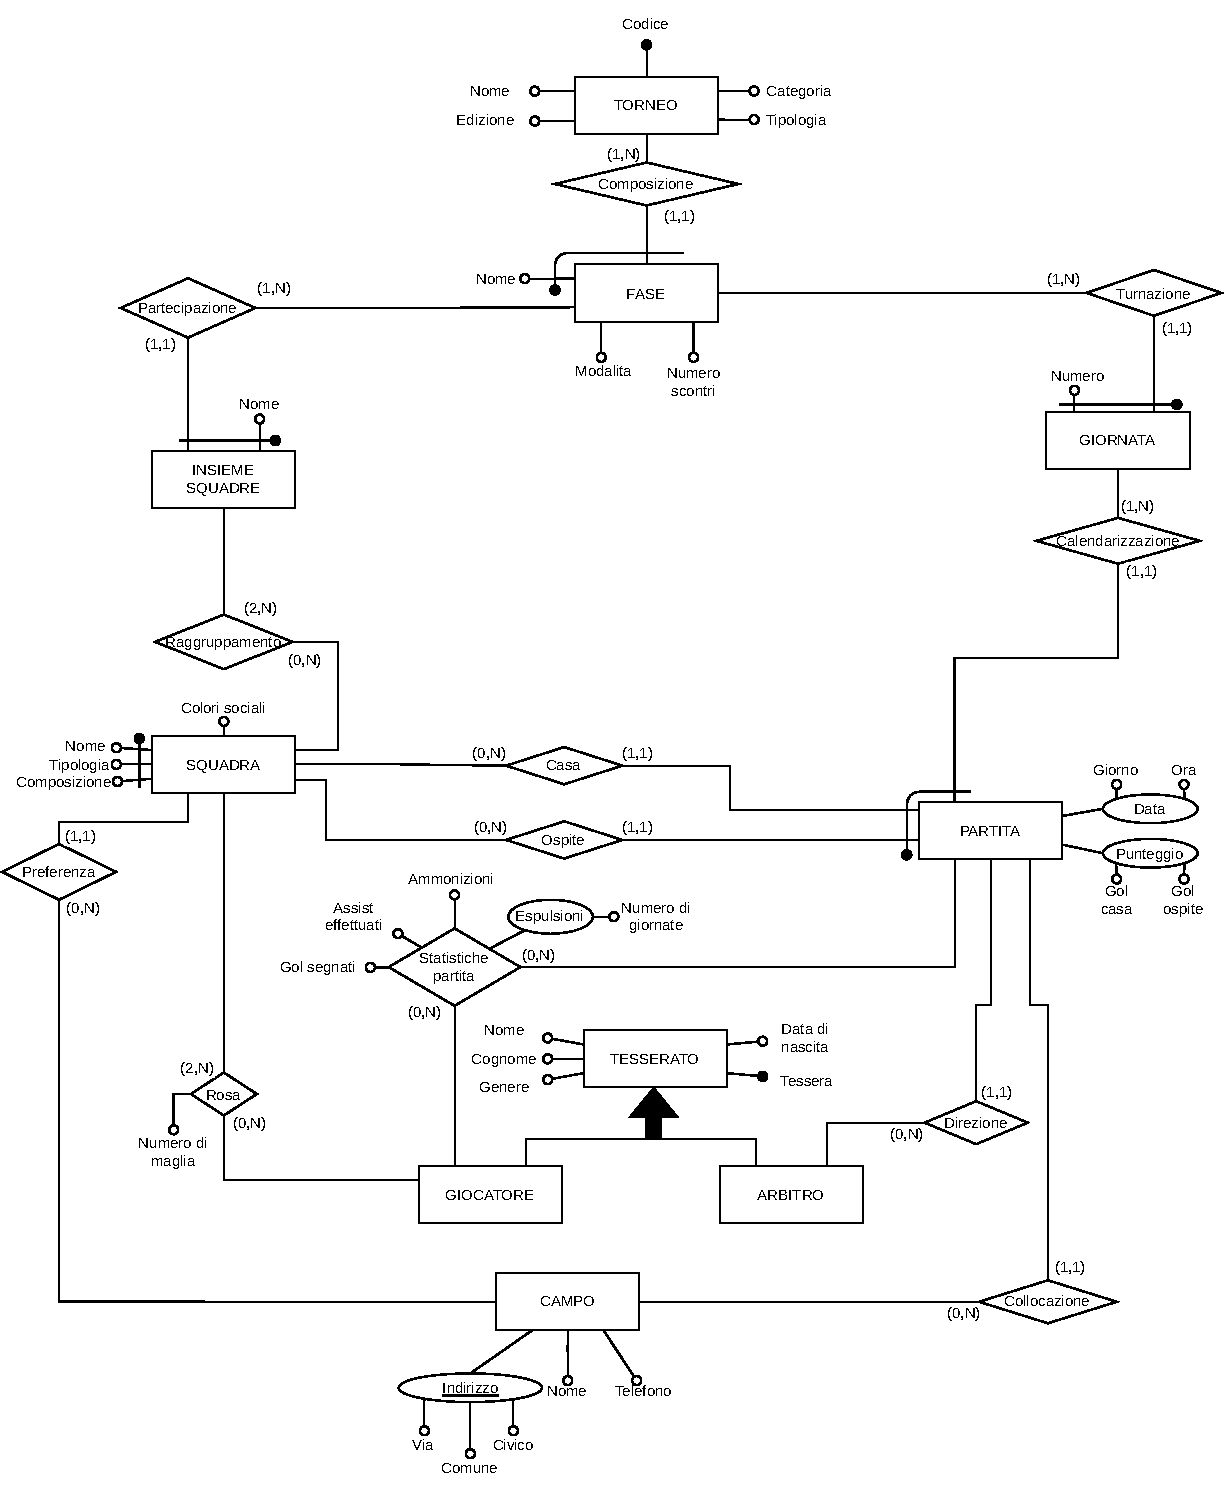
\includegraphics[scale=0.95, center]{./include/bdsi-prog-2023-ER.pdf}
				\label{fig:ER}
			\end{figure}
	\newpage		
	\part{Progettazione Logica}
		\section{Traduzione dello schema}
			\subsection{Eliminazione delle gerarchie}
				\underline{Concettuale} \hspace{7.5cm} \underline{Logico}\
				\begin{figure}[h]
					\begin{minipage}[b]{8.5cm}
						\centering
						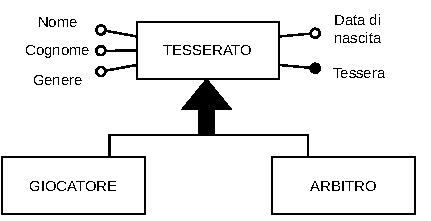
\includegraphics[width=8cm]{./include/bdsi-prog-2023-TRAD.C1.pdf}
					\end{minipage}
					\hspace{2mm} \hspace{3mm}
					\begin{minipage}[b]{8.5cm}
						\centering
						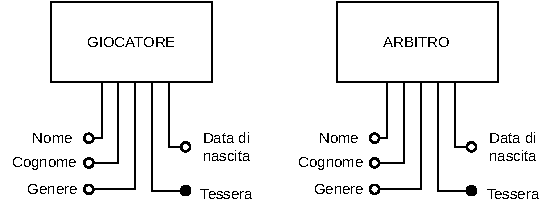
\includegraphics[width=9cm]{./include/bdsi-prog-2023-TRAD.L1.pdf}
					\end{minipage}
				\end{figure}
			\subsection{Eliminazione degli attributi multi-valore}
				\underline{Attributi composti partita}
				\begin{figure}[h]
					\begin{minipage}[b]{8.5cm}
						\centering
						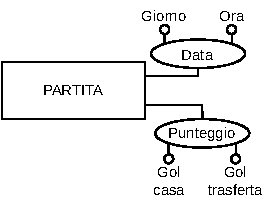
\includegraphics[width=5cm, height=2cm]{./include/bdsi-prog-2023-TRAD.C2.pdf}
					\end{minipage}
					\hspace{2mm} \hspace{3mm}
					\begin{minipage}[b]{8.5cm}
						\centering
						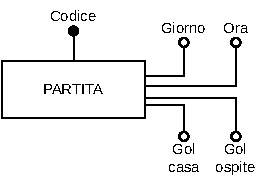
\includegraphics[width=5cm, height=3cm]{./include/bdsi-prog-2023-TRAD.L2.pdf}
					\end{minipage}
				\end{figure}
				
				\underline{Attributi composti campo}
				\begin{figure}[h]
					\begin{minipage}[b]{8.5cm}
						\centering
						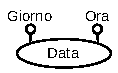
\includegraphics[width=4cm, height=2.5cm]{./include/bdsi-prog-2023-TRAD.C3.pdf}
					\end{minipage}
					\hspace{2mm} \hspace{3mm}
					\begin{minipage}[b]{8.5cm}
						\centering
						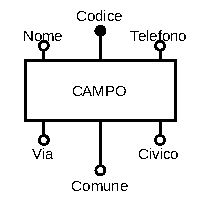
\includegraphics[width=4cm, height=3cm]{./include/bdsi-prog-2023-TRAD.L3.pdf}
					\end{minipage}
				\end{figure}
				
				\underline{Attributi composti statistiche partita}
				\begin{figure}[h!]
					\begin{minipage}[b]{8.5cm}
						\centering
						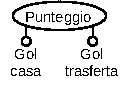
\includegraphics[width=4cm, height=1cm]{./include/bdsi-prog-2023-TRAD.C4.pdf}
					\end{minipage}
					\hspace{2mm} \hspace{3mm}
					\begin{minipage}[b]{8.5cm}
						\centering
						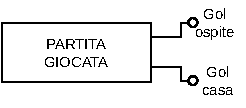
\includegraphics[width=6cm, height=2.5cm]{./include/bdsi-prog-2023-TRAD.L4.pdf}
					\end{minipage}
				\end{figure}
				

				
	

	\newpage
	\hrule
	\tableofcontents
	
\end{document}